%%%%%%%%%%%%%%%%%%%%%%%%%%%%%%%%%%%%%%%%%%%%%%%%%%%%%%%%%%%%%%%%%%%%%%%%%%%%
\documentclass[a4j,11pt]{jarticle}           % pLaTeX の場合
\usepackage{authblk}
\usepackage[dvipdfmx]{graphicx} 

% usepackage置場 TODO
\usepackage{cite}
%\usepackage[dvips]{graphicx}
\usepackage{amsmath}
\usepackage{amssymb}
\usepackage{marvosym}
\usepackage{pifont}
\usepackage{ascmac}
\usepackage{url}
\usepackage{booktabs}
\usepackage{float}
\usepackage{comment}
\newcommand{\argmin}{\mathop{\rm arg~min}\limits}
% \setlength{\oddsidemargin}{1.0cm}
% \setlength{\evensidemargin}{1.0cm}
\renewcommand{\floatpagefraction}{0.7}
\renewcommand{\baselinestretch}{1.3}
\renewcommand{\arraystretch}{0.8}
\renewcommand{\refname}{文献}
% \newcommand{\Nnm}{${\rm N_{n,m}}$}
\pagestyle{empty}
\bibliographystyle{prml}
%%%%%%%%%%%%%%%%%%%%%%%%%%%%%%%%%%%%%%%%%%%%%%%%%%%%%%%%%%%%%%%%%%%%%%%%%%%
\begin{document}
	\begin{titlepage}
		\setcounter{page}{0}
		\begin{center}
			\vspace*{2.0cm}
			\LARGE
			%タイトル
			ユーザーの好みに合ったモデルを用いた\\レコメンデーション\\
			\vfill
			%title(English)
			Personalized Recommendation by Models \\Fitting User Preference
			\vfill
			\LARGE
			北海道大学 工学部\\
			情報エレクトロニクス学科\\
			情報理工学コース\\
			情報認識学研究室
			
			\vspace{2ex}
			%名前
			茅根 宏介\\
			\vspace{2ex}
			%日付
			2020年3月\\
			\vspace*{2cm}
		\end{center}
	\end{titlepage}
	\tableofcontents \thispagestyle{empty}
	\newpage
	\listoffigures
	
	\listoftables
	\clearpage 
	\pagestyle{plain} 
	
	%%%%%%%%%%%%%%%%%%%%%%%%%%%%%%%%%%%%%%%%%%%%%%%%%%%%%%%%%%%%
	%platexでコンパイル
	%%%%%%%%%%%%%%%%%%%%%%%%%%%%%%%%%%%%%%%%%%%%%%%%%%%%%%%%%%%%
	
	\section{はじめに}
	\subsection{研究背景}
	推薦システムは, 近年多くのwebサービスにおいて使われており, ユーザにとって有用と思われるアイテムを, ユーザの目的に合った形で提示するシステムである\cite{rec1, rec2, rec3}. 最近では, Spotify\footnote{https://www.spotify.com/jp/}やNetflix\footnote{https://www.netflix.com/jp/}など, ソーシャルメディアを活用したサービスが普及し利用できる情報が増えた. 例えば, ソーシャルメディアでは, ユーザ同士が友好関係を作ったり, ユーザがアイテムにタグを付けることができる. これらのソーシャル情報は推薦システムにおいて有益であることが知られている\cite{social,tag}. ソーシャル情報などに含まれる様々なオブジェクト間の関係を表現する手法としてHeterogeneous Information Network (HIN)\cite{HIN}やハイパーグラフ\cite{hyper}がある. HINやハイパーグラフを用いた推薦手法ではユーザとアイテム間などの関係性をグラフを用いて表現し, 様々な類似性に基づいて推薦するため, 高精度のお勧めが可能である.
	
	\subsection{本論文の目的}
	ユーザのアイテムに対する評価のみでなくソーシャル情報などを用いて様々な類似性に基づく推薦を行うことができるハイパーグラフを用いた方法において, ランダムウォークを用いた推薦法に着目し, 推薦アイテムランキングへのユーザ, アイテム, タグなどの寄与分を変化させる方法を提案する. 本稿では, ユーザ, アイテム, タグなどを推薦因子とみなし, それらの推薦アイテムランキングへの寄与分は, ランダムウォークにおける定常分布において, それらに対応するノード集合の確率和であると考える. 推薦因子の寄与が異なるモデルによる推薦の精度を調べ, 最も精度の高いモデルがユーザ毎に異なることを検証する.	
	\subsection{本論文の構成}
	本論文は本節を含め全6節で構成する. 第2節ではソーシャル情報などに含まれるオブジェクト間の関係をグラフを用いて表す手法, および, それを用いた推薦システムを紹介する. 第3節では, 提案手法のベースとなる推薦手法であるMRHのリスタート付きランダムウォーク版を説明した後, 推薦因子の寄与分を定義し, それを変化させる方法として, ハイパーエッジの重みを変化させる方法を提案する. 第4節ではMRHのリスタート付きランダムウォーク版において定義される遷移確率行列が, ハイパーエッジの重みを変化させることによりどのように変わるかを確認する. 第5節では, 実データを用いてシミュレーションを行い, ハイパーエッジの重みの違いにより推薦因子の寄与分の違いが生じるのか, ユーザにより最適な重みのモデルが異なるのかを調べる. 最後に第6節では, 本論文の結論と今後の方針について述べる. 
	\newpage
	\section{多様な関係を表すグラフを用いた推薦}
	ソーシャル情報などを含めた様々なオブジェクト間の関係をグラフで表す2つの方法とそれらを用いた推薦システムを紹介する.
	\subsection{HINを用いた推薦}
	Heterogeneous Information Network (HIN)\cite{HIN}は, オブジェクト間の様々な関係性を, 複数の種類の辺を用いたグラフにより表現する手法である. 
	例えば, ユーザとアイテム間の購買関係や, ユーザ間の友人関係などは異なる種類の辺として表現される. HINは類似検索やクラスタリング, 分類問題などの分野において用いられている. 
	\\ Hete-CF\cite{Hete}は, HINを用いた推薦方式であり, ユーザ間, アイテム間, およびユーザとアイテム間の3つの関係を用いて類似性を求めて推薦している. 推薦モデルを最適化する際, それぞれの関係は重み付けされ, 重みを調整することで推薦モデルの精度を上げることが可能である. レーティング情報が少ない時, ユーザのアイテムに対する重みを大きくすることで精度が上がり, レーティング情報が多い時には偏りが生じてしまうのでその重みを小さくすることで精度が上がることが報告されている.
	\subsection{ハイパーグラフを用いた推薦}
	ハイパーグラフもHINと同様にオブジェクトの関係をグラフで表現したものであり, 3項以上の関係を表すハイパーエッジを用いるため, 対の関係よりも複雑な高次関係をモデル化できる. 従来よりクラスタリングや分類問題などの分野で利用されてきた\cite{hyper}. Music Recommendation via Hypergraph (MRH)\cite{MRH}は, ユーザがアイテムにつけたタグなど, ソーシャル情報などに含まれる3つ以上のオブジェクト間の関係をハイパーグラフを用いて表現し, 類似性を表すハイパーエッジの重みと各ユーザの好みを考慮した最適化問題を解くことにより, ユーザ毎にノードのランキングを行い推薦ランキングを生成する方式である. 論文\cite{MRH}では, バリエーションとして本稿で扱うリスタート付きランダムウォークモデルによるランキング計算法も提案している. MRHでは, ランキングを計算する際, 正規化された重みを使っており, 重みの調整に関する考察はされていない. 
	\newpage
	\section{提案手法}
	本稿では, 従来のハイパーグラフを用いた方法において, ユーザ, アイテム, タグなどのオブジェクトが推薦にどの程度寄与しているかを分析する指標, およびそれを変化させる方法を提案する. 提案手法は, MRH\cite{MRH}のリスタート付きランダムウォーク版をベースとしている. 最初にMRHにおけるハイパーグラフの構築法とリスタート付きランダムウォークについて説明し, その後にオブジェクトの推薦への寄与分を表す指標を定義し, それを変化させる方法を説明する.
	\subsection{ハイパーグラフ}
	ハイパーグラフ$G$は, 頂点集合$V=\{v_1,v_2,...,v_{|V|}\}$, ハイパーエッジの集合$E_h$, およびハイパーエッジの重み$w:E\rightarrow (0,\infty)$の3つ組$G(V,E_h,w)$で表される. ハイパーエッジ$e\in{E_h}$は, 通常のエッジを一般化したものであり, $V$の2ノード以上の部分集合である. ハイパーエッジ$e$の重み$w(e)$は, ハイパーエッジ$e$に含まれるオブジェクト間の類似度を表す. また, 頂点$V$およびハイパーエッジ$E_h$は多種類のものからなるとし, それぞれの種類の数をR, Sとする. 異なる種類の頂点, ハイパーエッジをそれぞれ$V^{(r)}(r=1,2,...,R)$, $E_h^{(s)}(s=1,2,...,S)$と表す. 例えばユーザの映画に対する評価情報とユーザが映画につけたタグ情報を利用した映画の推薦の場合, ノード集合$V$はユーザの集合$V^{(1)}$, 映画の集合$V^{(2)}$, タグの集合$V^{(3)}$の3種類のノード集合からなり, ハイパーエッジの集合$E_h$は評価情報のエッジ$E_h^{(1)}\in V^{(1)}\times V^{(2)}$とタグ情報のエッジ$E_h^{(2)}\in V^{(1)}\times V^{(2)}\times V^{(3)}$の2種類のエッジ集合からなるハイパーグラフを考える. 
	\\ 次に,  ハイパーグラフに関する行列表現を定義する. まず, 接続行列$\textbf{H}\in \{0, 1\}^{|V|\times |E_h|}$はノード$v$とエッジ$e$の関係を示し, Hの$(v, e)$成分を$h(v, e)$で表し, $v\in{e}$ならば$h(v, e)=1$, それ以外は$h(v, e)=0$と定義する. ハイパーエッジの重み行列$W_h$を, $(e, e)$成分が$w(e)$である$|E_h|\times |E_h|$の対角行列として定義する. さらに, ノード$v$の次数$d(v)$, ハイパーエッジ$e$の次数$\delta(e)$を,
	
	\begin{eqnarray}
	d(v)&=&\sum_{e\in E_h}w(e)h(v,e), \\ \delta(e)&=&\sum_{v\in V}h(v,e). 
	\end{eqnarray}
	と定義し, $(v, v)$成分を$d(v)$とする$|V|\times |V|$の対角行列を$\textbf{D}_v$, $(e, e)$成分を$\delta(e)$とする$|E_h|\times |E_h|$の対角行列を$\textbf{D}_e$とする.
	
	
	
	\subsection{RWRモデルによるランキング}
	Random walks with restarts model (RWR)\cite{rwr}は, リスタート付きランダムウォークの定常分布をランキングスコアとして用いる方法である. 時刻tにおけるグラフのノード集合$V$上の確率分布を$\textbf{f}^{(t)}$とする. $\textbf{f}^{(t)}$の初期確率分布およびリスタート確率分布として, ユーザの直接的な好みを表す分布$y\in[0,1]^{|V|}$を用いる. 実験で用いる$y$については第5.3節で述べる. リスタートを考慮しないランダムウォークの遷移確率行列Aとして$\textbf{A}=\textbf{D}_v^{-1}\textbf{H}\textbf{W}_h\textbf{D}_e^{-1}\textbf{H}^T$を用いる. このとき, Aの(i, j)成分$A_{i,j}$は, 
	\begin{equation}
	A_{i,j}=\sum_{s=1}^{S}\sum_{e\in E_h^{(s)}}\frac{w(e)h(v_i,e)h(v_j,e)}{\delta(e)d(v_i)}.
	\end{equation}
	と表せる. $A_{i,j}$は, オブジェクトiからみたオブジェクトjへの好みの類似度を表す値であり, ランダムウォークでは次の時刻に好みの類似するノードへ多く遷移する. リスタート確率を$\alpha$とすれば, リスタート付きランダムウォークにより, 確率分布$\textbf{f}^{(t)}$は以下の式で計算される確率分布$\textbf{f}^{(t+1)}$に変化する. 
	\begin{equation}
	\textbf{f}^{(t+1)}=(1-\alpha)\textbf{A}\textbf{f}^{(t)}+\alpha\textbf{y}.
	\end{equation}
	定常分布は, 定常時の恒等式より逆行列を計算してかけることにより得られるが, 高速計算のため式(4)を繰り返し適用することにより近似解を得る方法を用いる. 

	\subsection{推薦因子}
	第3.1節で定義したR種類のノード$V^{(r)}$を推薦因子とする. 用いたランダムウォークは好みの類似する方へ遷移するモデルであることから, 定常分布$\textbf{f}^*$における各オブジェクトの確率は, 好みの高さを示す値として用いることができる. この値は, 推薦オブジェクトにおいては, お勧めランキングに用いられるが, それ以外のオブジェクトにおいても, 全体が有向グラフとして連結であれば, 各お勧めアイテムに直接的および間接的に流れ入る割合を表していると考えられる. そこで各種のオブジェクトに対し, その種のオブジェクトの定常確率の合計を, お勧めアイテムランキングへのその種のオブジェクトの寄与度と定義する. 各種のオブジェクトの寄与分を変える事ができればユーザにとってより違いがわかりやすい推薦を提示できる.
	
	\subsection{エッジの種毎に重みを変えた推薦}
	各オブジェクトの寄与分を直接調整することは困難である. そこで, オブジェクトに関連するハイパーエッジの重みを変化させることにより, そのオブジェクトの寄与分を変化させる. RWRモデルにおいてハイパーグラフのエッジの重みを自由に変えても遷移確率行列としての性質が維持されることに注意する. 各ハイパーエッジの種類毎に, その種のエッジの重みを重視したモデルを構築し, 各ユーザに対して異なるお勧めを計算する.
	\newpage
	\section{重みを変えることによる遷移行列の変化}
	推薦因子の寄与分が変わるためには, まず, 遷移確率行列\textbf{A}が変わる必要がある. この節では, ハイパーエッジの重みを変えることにより遷移確率行列\textbf{A}がどのように変わるのか分析する. 重みを大きくする種のエッジを$E_h^{(t)}$とし, 重みを$\alpha$倍すると
	\begin{eqnarray}
	A_{i,j}=\frac{1}{d(v_i)}&\Bigl(&\sum_{s\neq t}\sum_{e\in E_h^{(s)}}\frac{w(e)h(v_i,e)h(v_j,e)}{\delta(e)} \nonumber\\ &+&\alpha\sum_{e\in E_h^{(t)}}\frac{w(e)h(v_i,e)h(v_j,e)}{\delta(e)}\Bigr). 
	\end{eqnarray}	
	となる. ただし$d(v_i)$も大きくなり
	
	\begin{equation}
	d(v_i)=\sum_{s\neq t}\sum_{e\in E_h^{(s)}}w(e)h(v_i,e)+\alpha\sum_{e\in E_h^{(t)}}w(e)h(v_i,e). 
	\end{equation}
	となる. したがって, $v_i$を含むエッジが$E_h^{(t)}$にない場合は$\textbf{A}_{i,j}$は変化しない. $v_i$を含むエッジが$E_h^{(t)}$にある場合, $\{v_i, v_j\}$を含むエッジが$E_h^{(t)}$になければ$\textbf{A}_{i,j}$の重みは小さくなり, $\alpha \rightarrow \infty$とすれば0に収束する. $\{v_i, v_j\}$を含むエッジが$E_h^{(t)}$にある場合は,
	
	\begin{eqnarray}
	a &=& \frac{\sum_{s\neq t}\sum_{e\in E_h^{(s)}}\frac{w(e)h(v_i,e)h(v_j,e)}{\delta(e)}}{\sum_{s\neq t}\sum_{e\in E_h^{(s)}}w(e)h(v_i,e)}, \\
	b &=& \frac{\sum_{e\in E_h^{(t)}}\frac{w(e)h(v_i,e)h(v_j,e)}{\delta(e)}}{\sum_{e\in E_h^{(t)}}w(e)h(v_i,e)}.
	\end{eqnarray}
	
	とすれば, $a>b$のときは$\textbf{A}_{i,j}$は減少, $a<b$のときは$\textbf{A}_{i,j}$は増加し, $\alpha \rightarrow \infty$とすれば, いずれもbに収束する.
	\newpage
	\section{実験}
	第4節で述べたように, ハイパーエッジの重みを調整することで推薦因子の寄与分を変えることが可能か, また, 推薦因子の寄与が異なるモデルによる精度を比較において, ユーザ毎に最も精度の高いモデルが異なるか, 実データを用いたシミュレーションにより調査する.
	\subsection{データセット}
	MovieLensデータセット(MovieLens Latest Datasets\footnote{https://grouplens.org/datasets/movielens/})を用いる. 1から5の5段階で評価された評価値と, 映画に対してユーザが付けたタグ情報を使ってハイパーグラフを構築した. オブジェクトおよび関係性のデータ数を表1に示す.%ciao\footnote{https://www.ciao.co.uk}, ciaoも同様にユーザがアイテムにレーティングをつけるレビューサイトであり, ユーザ同士で友好関係を作ることができる. それぞれのオブジェクトや関係性の詳細を以下に示す. 
	
	\begin{table}[H]
		\centering
		\caption{MovieLensデータセットのオブジェクトおよび関係性のデータ数}
		\begin{tabular}{ccccc}\hline
			&\multicolumn{2}{c}{オブジェクト}&\multicolumn{2}{c}{関係性} \\
			&種類&数&種類&数 \\ \hline
			&ユーザ(U)&610&評価値(U, M)&100836\\
			MovieLens&映画(M)&9742&タグ情報(U, M, T)&3683\\
			&タグ(T)&1589\\ \hline
			%ciao&ユーザ(U)&7375&評価値(U, M)&284086\\
			%&アイテム(M)&106797&友人情報(U, U)&111781\\ \hline
		\end{tabular}
	\end{table}
	
	\subsection{ハイパーグラフの構築}
	MovieLensのデータセットを用いて, ユーザ($\textbf{U}$), 映画($\textbf{M}$), タグ($\textbf{T}$)の3種のオブジェクト(R=3)とそれらの関係を表す2種のハイパーエッジ(S=2)をもつハイパーグラフを構築する. $E_h^{(s)}$の正規化された重みは論文\cite{MRH}に従い次のように決定する. 
	\\\\(i) $E_h^{(1)}$: ユーザ$u_i$が評価値を付けた映画$m_j$のペア$e^{(1)}_{ij}=\{u_i,m_j\}$の集合. 重み$w(e_{ij}^{(1)})$はユーザが映画につけた評価値(1$\sim$5)とする. 正規化した重み$w(e_{ij}^{(1)})^*$は, ユーザ, 映画に対する偏りを補正した重み$w(e_{ij}^{(1)})'$を他の種類のエッジと同等に扱うために$w(e_{i1}^{(1)})',...,w(e_{i|M|}^{(1)})'$の平均$ave(w(e_i^{(1)})')$で割って正規化したもので以下のように定義する.
	
	\begin{equation}
	w(e_{ij}^{(1)})'=\frac{w(e_{ij}^{(1)})}{\sqrt{\sum_{k=1}^{|M|}w(e_{ik}^{(1)})}\sqrt{\sum_{l=1}^{|U|}w(e_{lj}^{(1)})}},
	\end{equation}
	
	
	\begin{equation}
	w(e_{ij}^{(1)})^*=\frac{w(e_{ij}^{(1)})'}{ave(w(e_i^{(1)})')}.
	\end{equation}
	(ii) $E_h^{(2)}$: ユーザ$u_i$が映画$m_j$に対して付けたタグ$t_h$の3つ組$e^{(2)}_{ijh}=\{u_i,m_j,t_h\}$の集合. 重み$w(e_{ijh}^{(2)})$は1. 
	\subsection{実験設定}
	各ハイパーエッジの重みを無限大にして計算した重みと正規化した重みのモデルを用い, リスタート付きランダムウォークモデルで定常分布を求め, 異なる重みを用いたモデルにおける, 各オブジェクトの寄与分およびランキング精度の比較を行う. 定常分布を求めるための式(4)の繰り返しは80回に固定する.\footnote{収束判定は, 十分小さな$\epsilon$に対し$||f^{(t+1)}−f^{(t)} || < \epsilon$で行うなどすべきであるが, fは数回で急速に変化し, 残りのステップでは比較的安定してくることが実験により確認されたため, 今回は80回に固定した. }リスタート確率$\alpha$は0.04とした. ユーザの直接的な好みを表す分布$y$は, MRH\cite{MRH}で提案されている方法の1つを採用し, おすすめするターゲットユーザ$u_i$に対し, \textbf{A}のi行目$A_{i,*}^T$を用いる.
	\subsection{評価指標}
	評価指標としてランキング予測結果の評価指標として広く用いられているNormalized Discount Cumulative Gain (NDCG)を用いる. NDCGは, 下位に行くほどスコアを割引して計算するランキング評価指標であるDiscounted Cumulative Gain (DCG)を, 真の評価値ランキングに対するDCG (Ideal DCG (IDCG))で割ることで正規化した指標である. NDCGは0から1の値を取り, 1に近いほど精度がよいことを示す. ターゲットユーザuに対してモデルAを用いて求めたNDCGは
	\begin{equation}
	NDCG@n(A,u)=\frac{1}{IDCG}\times\sum_{i=1}^n\frac{2^{r_i}-1}{\log_2(i+1)}.
	\end{equation}
	と定義される. $r_i$はモデルAにおいてランキングi位の要素に対する評価値であり, nは評価に用いる要素数を表す. 評価値は, トレーニングデータを用いて定常分布を求めた後, テストデータにおけるランキングスコアが高い上位n個の映画の評価値を用いる. 
	\\ また, モデルを変えることで1ユーザあたりどのくらい精度が変化するのかをMAND (Mean Absolute NDCG Difference)により調査する. 
	第5.2節で定義した正規化された重みのモデル$(A_1)$とエッジの重さを大きくした他モデル$(A_2)$間での, 各ユーザの精度がどのくらい異なるのかを検証する. 
	ユーザ数をmとすると2つのモデル間におけるMANDは以下のように表される. 
	\begin{eqnarray}
	MAND(A_1,A_2)=\frac{1}{m}\sum_{u=1}^m|&NDCG@n(A_1,u)& \nonumber\\-&NDCG@n(A_2,u)&|.
	\end{eqnarray}
	
	\subsection{実験結果}
	\subsubsection{推薦因子の寄与分}
	各モデルの定常分布$\textbf{f}^*$における推薦因子の寄与分図1に示す. グラフには全ユーザに対する平均の値が示されている. 
	\begin{comment}

	\begin{table}[H]
		\centering
		\caption{推薦因子の寄与分[\%]}
		\begin{tabular}{ccc}\hline
			&MovieLens(U, M, T)  \\ \hline
			正規化& 38.6 \ / 37.2 \ / 24.2  \\ 
			評価値& 50.7 \ / 49.3 \ / 0.0  \\
			タグ情報&  37.5 \ / 36.2\ / 26.2 \\ \hline
		\end{tabular}
	\end{table}
	\end{comment}

	\begin{figure}[H]
		\centering
		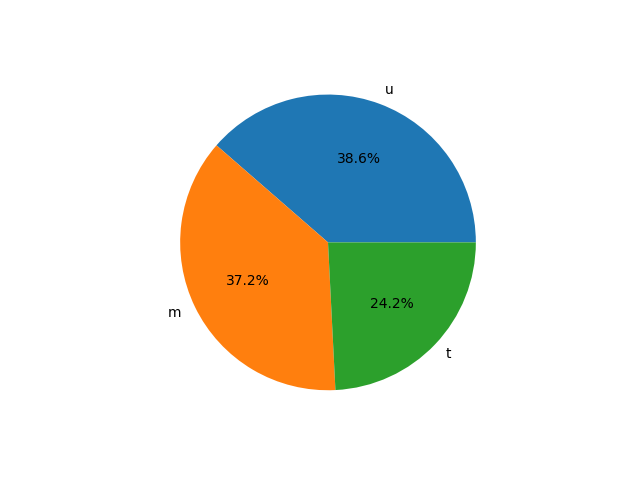
\includegraphics[bb=0 0 360 270, width=\hsize]{img/Figure_1.png}
	\end{figure}
	
	\begin{figure}[h]
		\centering
		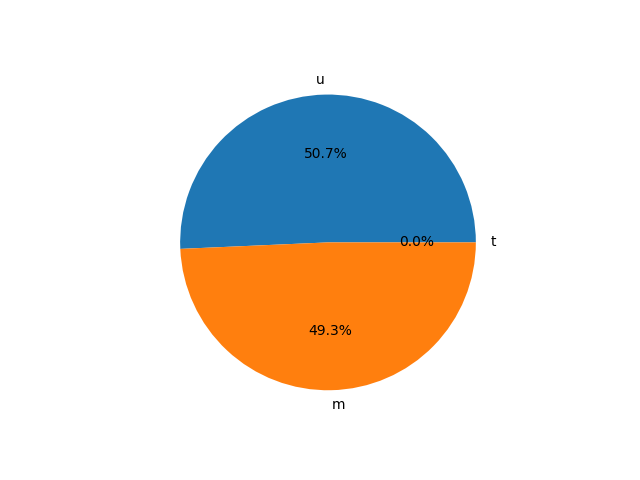
\includegraphics[bb=0 0 360 270, width=\hsize]{img/Figure_2.png}
	\end{figure}
	\begin{figure}[H]
		\centering
		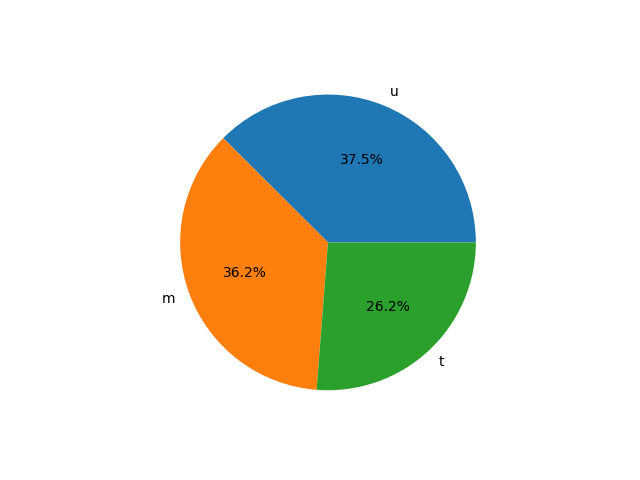
\includegraphics[bb=0 0 360 270, width=\hsize]{img/Figure_3.png}
		\caption{各モデルにおける推薦因子の寄与分. 上段: 正規化 中段: 評価値 下段: タグ情報 }
	\end{figure}

	\begin{comment}
	
	\begin{table}[H]
	\centering
	\caption{推薦因子の寄与分[\%]}
	\begin{tabular}{ccc}\hline
	&movielens(U, M, T)  &ciao(U, M) \\ \hline
	正規化& 38.6 \ / 37.2 \ / 24.2 &  64.6 \ / 35.4 \\ 
	評価値& 50.7 \ / 49.3 \ / 0.0 &  50.7 \ / 49.3 \\
	タグ情報, 友人関係 &  37.5 \ / 36.2\ / 26.2 &  100.0 \ / 0.0\\ \hline
	\end{tabular}
	\end{table}
	\end{comment}
	図1から, 関係性を表現するエッジの重みを大きくすることで, 推薦結果における推薦因子の寄与分が異なるモデルを構築できたことがわかる. %しかし, あるエッジの重みを大きくすることで, 必ずそのエッジの依存度が上がり, エッジが含む推薦因子の寄与分を大きくできるわけではないことがわかった. 第4節で検証したように関係性を表現するエッジの重みを大きくすることによる推薦因子の寄与分の変化の仕方はデータ依存であることがわかった. 
	\subsubsection{推薦の精度}
	ユーザ毎に推薦因子の寄与が異なるモデルによる精度を比較するために, ユーザを最も高い精度を出したモデルごとにグループ分けした. それぞれのグループにおける各モデルの精度を表2に示す.
	
	\begin{table}[H]
		\caption{NDCG@20の比較}
		{
			\scalebox{0.8}{
				\begin{tabular}{ccccc}\hline
					グループ(人数)&全員(610)&正規化(221)&評価値(177)&タグ情報(212)\\ \hline
					NDCG(正規化)&0.758&\textbf{0.789}&0.752&0.730\\ 
					NDCG(評価値)&0.756&0.753&\textbf{0.793}&0.730\\
					NDCG(タグ情報)&0.758&0.753&0.749&\textbf{0.770}\\ \hline
				\end{tabular}
			}
		}
	\end{table}
	\begin{comment}
	
	\begin{table}[H]
	\caption{ciaoにおけるNDCG@20の比較}
	{
	\scalebox{0.8}{
	\begin{tabular}{ccccc}\hline
	グループ(人数)&全員(7375)&正規化(3716)&評価値(1765)&友人関係(1894)\\ \hline
	NDCG(正規化)&0.892&\textbf{0.926}&0.877&0.873\\ 
	NDCG(評価値)&0.892&0.892&\textbf{0.915}&0.872\\
	NDCG(友人関係)&0.894&0.891&0.876&\textbf{0.915}\\ \hline
	\end{tabular}
	}
	}
	\end{table}
	\end{comment}
	表2より, このデータセットではモデルを変えても全ユーザに対しての精度はほとんど変わらない. 太字は各グループにおいてそれぞれ最適なモデルで推薦した場合の精度である. 正規化したモデルにおける精度と比較した時, 精度が大きく向上していることが確認できる. 
	\\ また, 評価値, タグの重みを無限大にしたモデルの, 正規化された重みのモデルに対して計算したMANDを表3に示す. 
	
	\begin{table}[H]
		\centering
		\caption{正規化されたモデルと他モデル間におけるMAND}
		\begin{tabular}{cc}\hline
			MAND(評価値)&MAND(タグ情報) \\ \hline
			0.035&0.034 \\ \hline
		\end{tabular}
	\end{table}
	\begin{comment}
	
	
	\begin{table}[H]
	\centering
	\caption{ciaoにおける正規化したと他モデル間におけるMAND}
	\begin{tabular}{cc}\hline
	MAND(評価値)&MAND(友人関係) \\ \hline
	0.032&0.034 \\ \hline
	\end{tabular}
	\end{table}
	\end{comment}
	表3のMANDを見ると約0.034の違いがあることから, 3つのモデルではランキングがある程度異なることが確認できた. 
	\\ 	推薦モデルを変えることで上位20個の推薦リストがどう変わるのか全ユーザに対する平均を調査した. 正規化されたモデルと比較して, 評価値のモデルでは約8個, タグ情報のモデルでは約1個異なるアイテムが含まれていた. 例として3名のユーザに対する推薦リスト(ランキング10
	位まで)を表4に示す.
	
	
	
	\begin{table}[H]
		\caption{Top10の推薦リスト}
		{
			\scalebox{0.6}{
				\begin{tabular}{llll}\hline
					UserID&正規化&評価値&タグ情報 \\ \hline
					1 & 924:A Space Odyssey &318:Shawshank Redemption&7020:Proof \\
					&293:Léon&589:Terminator&924:A Space Odyssey \\
					&7361:Eternal Sunshine of the Spotless Mind&150:Apollo 13&293:Léon \\
					&4878:Donnie Darko&32:Twelve Monkeys&7361:Eternal Sunshine of the Spotless Mind \\
					&79132:Inception&380:True Lies&4878:Donnie Darko \\
					&72998:Avatar&588:Aladdin&79132:Inception \\
					&135536:Suicide Squad&858:Godfather&72998:Avatar \\
					&1921:Pi&377:Speed&135536:Suicide Squad  \\
					&3676:Eraserhead&165:Die Hard: With a Vengeance&1921:Pi  \\
					&4226:Memento&364:Lion King&3676:Eraserhead  \\ \hline 
					132&924:A Space Odyssey &110:Braveheart &924:A Space Odyssey \\
					&6327:Decade Under the Influence &527:Schindler's List &6327:Decade Under the Influence \\
					&72998:Avatar &150:Apollo 13 &72998:Avatar \\
					&1921:Pi &480:Jurassic Park &1921:Pi \\
					&135536:Suicide Squad &589:Terminator  &3676:Eraserhead \\
					&3676:Eraserhead &457:Fugitive &7932:Dark Days \\
					&4144:In the Mood For Love &590:Dances with Wolves &135536:Suicide Squad  \\
					&541:Blade Runner &1198:Raiders of the Lost Ark &4144:In the Mood For Love \\
					&2762:Sixth Sense &780:Independence Day &541:Blade Runne \\
					&122912:Avengers: Infinity War &608:Fargo  &2762:Sixth Sense\\ \hline
					606&7936:Shame  &150:Apollo 13 &7936:Shame \\
					&135536:Suicide Squad &457:Fugitive &135536:Suicide Squad \\
					&4878:Donnie Darko &608:Fargo &1288:This Is Spinal Tap  \\
					&79132:Inception &380:True Lies &4223:Enemy at the Gates \\
					&1288:This Is Spinal Tap &588:Aladdin  &112552:Whiplash \\
					&112552:Whiplash &377:Speed &4878:Donnie Darko \\
					&4223:Enemy at the Gates &364:Lion King &79132:Inception \\
					&122912:Avengers: Infinity War &595:Beauty and the Beast &122912:Avengers: Infinity War \\
					&99114:Django Unchained &344:Ace Ventura: Pet Detective &6235:Europa Europa \\
					&6235:Europa Europa &165:Die Hard &99114:Django Unchained \\ \hline
				\end{tabular}
			}
		}
	\end{table}
	
	\newpage
	\section{おわりに}
	本論文では, ユーザのアイテムに対する評価のみでなくソーシャル情報などを用いて様々な類似性に基づく推薦を行うことができるハイパーグラフを用いた方法において, ランダムウォークを用いた推薦法に着目し, 推薦結果におけるユーザ, アイテム, タグなどの推薦因子の寄与分を変化させる方法を提案した. 検証実験の結果によれば, 推薦因子の寄与分が異なるモデル間において, ユーザによって最適な推薦モデルが異なることが分かった. \\ 今後の課題として, 推薦因子の寄与分の有効な活用法やユーザの重みの学習法の開発が挙げられる.
	
	\newpage
	\section*{謝辞}
	\addcontentsline{toc}{section}{\numberline{}謝辞}
	本研究を行うにあたり,北海道大学大学院情報科学研究科情報理工学専攻数理科学講座
	情報認識学研究室の中村篤祥准教授には,研究テーマの設定から方針,内容について貴重
	な教示を賜りましたことを,深く御礼申し上げます.また,工藤峰一教授には貴重な御意見を頂きましたことを深く御礼申し上げます.最後に,同研究室の先輩方には
	研究や発表を含め様々な御指導, 御協力に感謝致します. 
	\newpage
	%\section*{参考文献}
	\small
	\addcontentsline{toc}{section}{\numberline{}文献}
	\bibliography{ref}	


\end{document}
